\subsection{Traffic Control}

\begin{frame}{Packet Scheduling}
	\begin{itemize}
		\item On complex systems, thousands of applications may use the same interface
		\item The scheduling of egress traffic needs to be configurable and predicatble
		\item Queueing strategies can be tunes for \textbf{throughput} and \textbf{latency}
		\item \textbf{tc} is the main component that deals with traffic scheduling
	\end{itemize}
\end{frame}

\begin{frame}{Packet Scheduling in the stack}
	\begin{columns}
		\column{0.4\textwidth}
		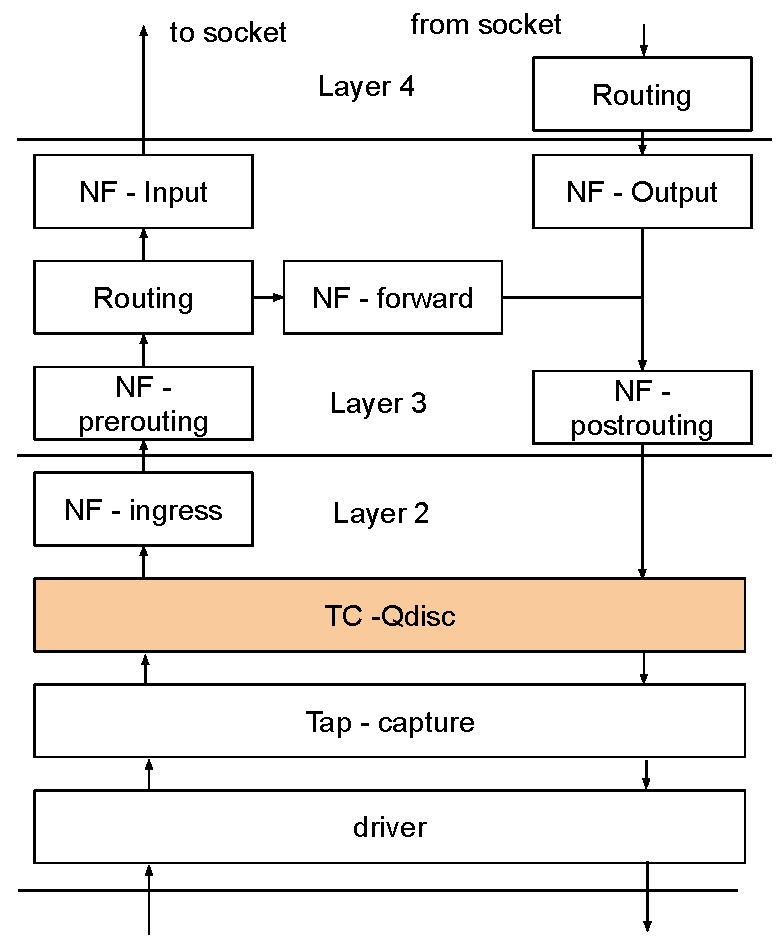
\includegraphics[width=1\textwidth]{slides/networking-traffic-control/routing_tc.pdf}
		\column{0.6\textwidth}
		\begin{itemize}
			\item The scheduling decision occurs between \textbf{routing} and the \textbf{driver}
			\item On \textbf{egress}, decides which packet to enqueue
			\item On \textbf{ingress}, may decide to drop or redirect
		\end{itemize}
	\end{columns}
\end{frame}

\begin{frame}{TC : Traffic Control}
	\begin{itemize}
		\item \code{tc} is a subsystem in charge of traffic control operations, namely :
			\begin{itemize}
				\item \textbf{Traffic Shaping} : Control the transmission rate for traffic classes
				\item \textbf{Traffic Scheduling} : Control the ordering and burst behaviour of outgoing traffic
				\item \textbf{Traffic Policing} : Control the reception rate for traffic classes
				\item \textbf{Drop control} : Control discard conditions for egress and ingress traffic
				\item \textbf{Classification} : Identify packets of interest for further actions
			\end{itemize}
	\end{itemize}
\end{frame}

\begin{frame}{TC use-cases}
	\begin{itemize}
		\item \code{tc mqprio} - Assign priorities to the Network Controller's queues
		\item \code{tc taprio} - Time-aware queue priorisation, for TSN
		\item \code{tc flower} - Flow-based actions, can be offloaded to hardware
		\item \code{tc ingress} - Attach TC actions to ingress traffic
	\end{itemize}
\end{frame}

\begin{frame}{TC QDisc : Queueing Disciplines}
	\begin{itemize}
		\item Controls how traffic is enqueued, in the \textbf{tx} direction
		\item Allows shaping the traffic very precisely on a per flow basis
		\item \textbf{Flows} can be assigned different \textbf{Qdisc} to define how to schedule transmission
	\end{itemize}
\end{frame}

\begin{frame}{Queues}
	\begin{itemize}
		\item Queue management is crucial for Lantency and Throughput
		\item Long queues allows absorbing network instabilities...
		\item ... but may cause to latencies, leading to \textbf{bufferbloat}
		\item The Network Interface's queues are exposed to TC
		\item \textbf{qdisc} algorithms select which queue is used for a given \textbf{flow}
	\end{itemize}
\end{frame}

\begin{frame}{Traffic flows}
	\begin{itemize}
		\item Packets with same \textbf{addressing parameters} are part of the same \textbf{flow}
		\item A Layer 4 flow is defined by 4 parameters : It's a \textbf{4-tuple}
			\begin{itemize}
				\item Source and Destination \textbf{ports}
				\item Source and Destination \textbf{IP address}
			\end{itemize}
		\item A Layer 3 flow is defined by 2 parameters : It's a \textbf{2-tuple}
			\begin{itemize}
				\item Source and Destination \textbf{IP address}
			\end{itemize}
		\item The \textbf{vlan id}, if applicable, may be included in the flow definition
			\begin{itemize}
				\item FLows may thefore be \textbf{3-tuple} or \textbf{5-tuple}
			\end{itemize}
		\item When acting on a packet, we need to identify the \textbf{flow} it belongs to :
		\item This is called \textbf{n-tuple classification}. The \code{n-tuple} is extracted, and its \textbf{hash} is computed
		\item Extracting the \code{n-tuple} value from a packet is called \textbf{bissection}
		\item The hash is used for the subsequent lookup operations, and may be computed in hardware.
	\end{itemize}
\end{frame}

\begin{frame}{TC example : QDisc}
	\begin{columns}
		\column{0.3\textwidth}
		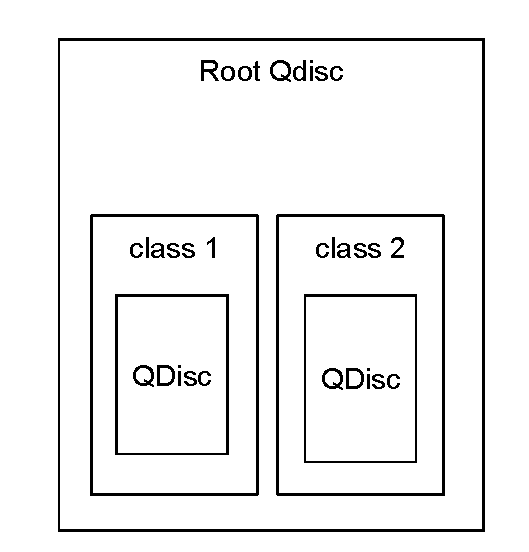
\includegraphics[width=\textwidth]{slides/networking-traffic-control/tc-qdisc.pdf}
		\column{0.7\textwidth}
		\begin{itemize}
			\item Queueing Disciplines, or \textbf{qdisc}, allow configuring the queue policy
			\item Multiple qdisc can co-exist, separated in diffent \textbf{classes}
			\item \textbf{classes} are used to split traffic, and enforce policing
			\item Traffic is assigned to classes through \textbf{classification}
		\end{itemize}
	\end{columns}
\end{frame}

\begin{frame}[fragile]{TC example : Classification}
	\begin{itemize}
		\item Match traffic with priority 0 or 4, and assign it to class "1:20"
	\begin{minted}{bash}
tc filter add dev eth0 parent 1: basic match 'meta(priority eq 0)' \
or 'meta(priority eq 4)' classid 1:20
	\end{minted}
		\item In \textbf{ingress}, classification is usually done to assign traffic to queues
		\item It can also be used for early filtering : \begin{minted}{bash}
tc qdisc add dev eth0 ingress
tc filter add dev eth0 protocol ip parent ffff: flower \
ip_proto tcp dst_port 80 \
action drop
\end{minted}
	\item \code{tc-flower} can also be offloaded to hardware, see \manpage{tc-flower}{8}
	\end{itemize}
\end{frame}

\begin{frame}[fragile]{TC example : shaping}
	\begin{itemize}
		\item Traffic Shaping, consists in limiting the egress rate of a flow
		\item Multiple strategies exist :
			\begin{itemize}
				\item Add Jitter on purpose : \code{tc qdisc add dev eth0 root netem delay 10ms 5ms}
				\item Use a Token Bucket filter : \code{tc qdisc add dev eth0 parent 1:1 handle 10: tbf rate 256kbit}
			\end{itemize}
		\item This can be combined with classification :
			\begin{minted}{bash}
tc qdisc add dev eth0 root handle 1: prio
tc qdisc add dev eth0 parent 1:3 handle 30: tbf rate 250kbit
tc filter add dev eth0 protocol ip parent 1:0 prio 3 u32 match ip \
dst 192.168.42.2/32 flowid 1:3
			\end{minted}
	\end{itemize}
\end{frame}

\begin{frame}[fragile]{TC example : editing}
	\begin{itemize}
		\item TC also allows editing traffic or metadata on-the-fly
		\item This is done with the \code{skbedit} action
		\item This can be used to change the \code{skb->priority} field
		\item Can also control which Hardware \textbf{tx queue} will be used
	\end{itemize}
	\begin{minted}{bash}
tc filter add dev eth0 parent 1: protocol ip prio 1 u32 \
match ip dst 192.168.0.3 \
action skbedit priority 6
	\end{minted}
\end{frame}

\begin{frame}{TC mqprio}
	\begin{columns}
	\column{0.3\textwidth}
		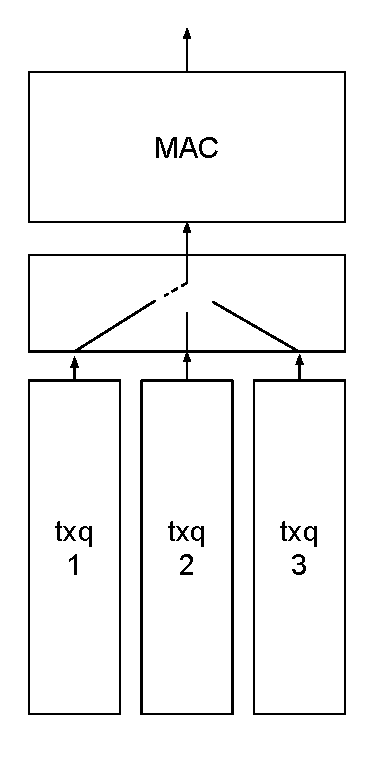
\includegraphics[width=0.8\textwidth]{slides/networking-traffic-control/txq_mq.pdf}
	\column{0.7\textwidth}
	\begin{itemize}
		\item Most Network Controllers today have mutilple queues in \code{tx} and \code{rx}
		\item They implement in hardware a \textbf{policing} algorithmm to select the next \code{tx} queue to use
			\begin{itemize}
				\item It can be a simple \textbf{weighted round robin} algorithm
				\item Alternatively a \textbf{strict priority} selection
				\item Some controllers also implement Time-aware scheduling for queue selection
			\end{itemize}
	\end{itemize}
	\end{columns}
\end{frame}

\begin{frame}{TC mqprio}
	\begin{center}
		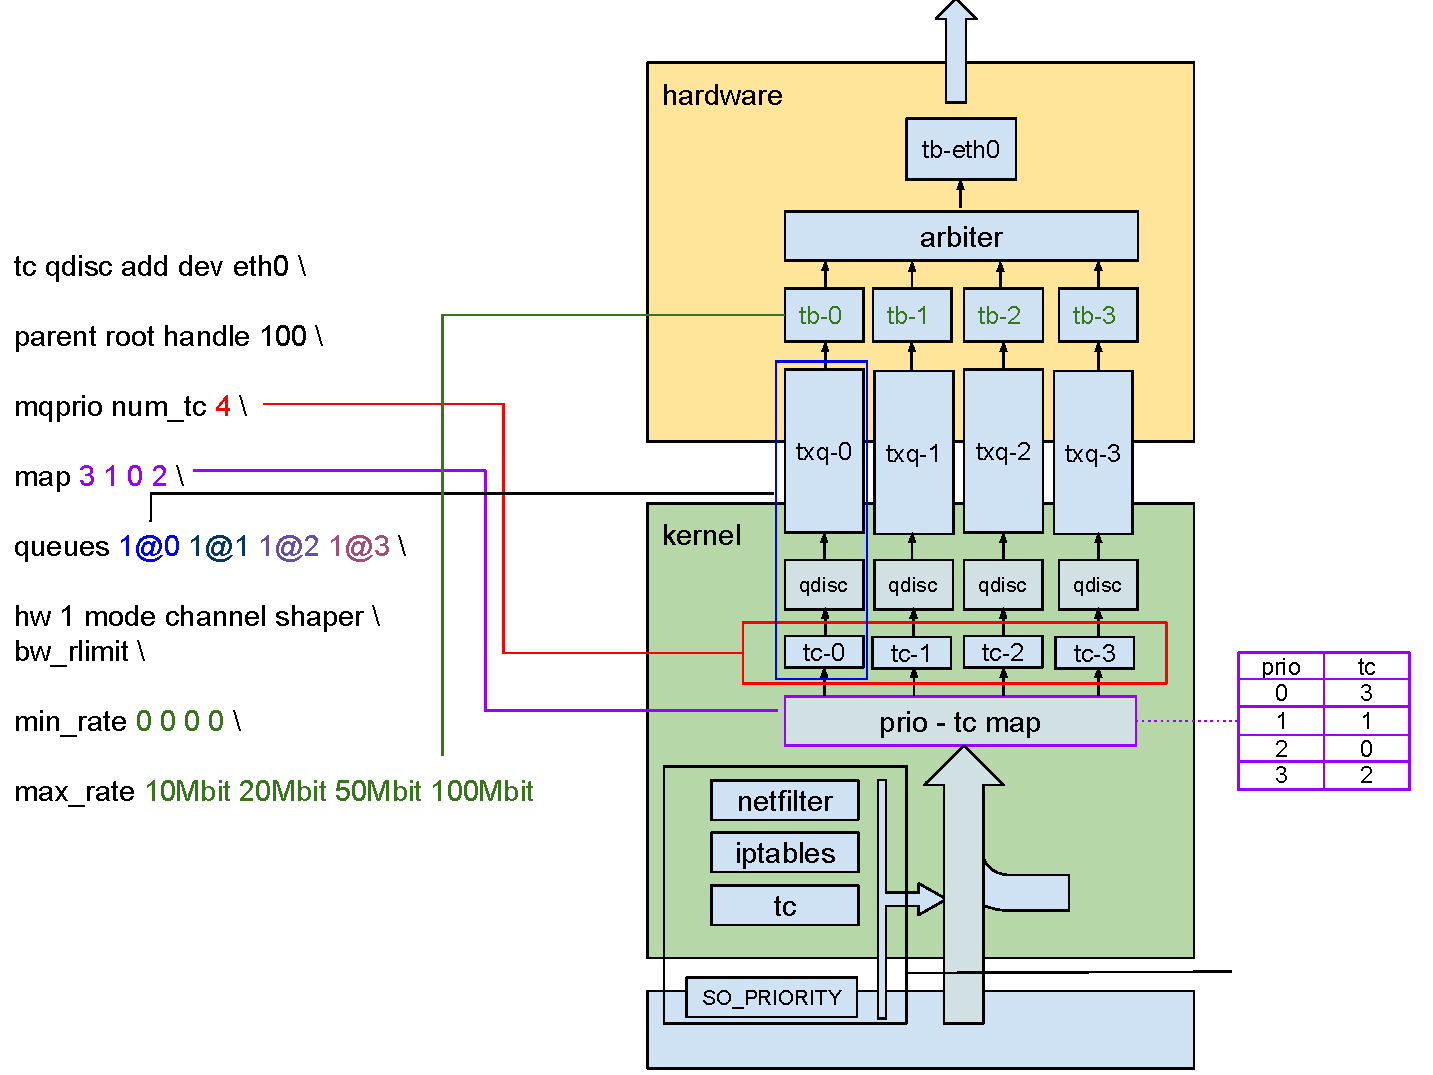
\includegraphics[width=0.8\textwidth]{slides/networking-traffic-control/TX_path_tc_mqprio.pdf}
	\end{center}
\end{frame}

\begin{frame}{TC offloads}
	\begin{itemize}
		\item Some TC operations can be offloaded to the Ethernet Controler, if supported
		\item \code{tc mqprio} - The Hardware will implement the queue-selectin algorithm
		\item \code{tc taprio} - For TSN-enabled hardware
		\item \code{tc flower} - Classication in \textbf{ingress} is done by hardware
	\end{itemize}
\end{frame}

% netfilter, iptables et. al.

